\documentclass[a4paper]{article} 
\usepackage{amsmath,amsfonts,bm}
\usepackage{hyperref}
\usepackage{amsthm} 
\usepackage{geometry}
\usepackage{amssymb}
\usepackage{pstricks-add}
\usepackage{framed,mdframed}
\usepackage{graphicx,color} 
\usepackage{mathrsfs,xcolor} 
\usepackage[all]{xy}
\usepackage{fancybox} 
\usepackage{xeCJK}
\newtheorem*{theorem}{定理}
\newtheorem*{remark}{注}
\newtheorem*{lemma}{引理}
\newtheorem*{corollary}{推论}
\newtheorem*{exercise}{习题}
\newtheorem*{example}{例}
\geometry{left=2.5cm,right=2.5cm,top=2.5cm,bottom=2.5cm}
\setCJKmainfont[BoldFont=Adobe Heiti Std R]{Adobe Song Std L}
\renewcommand{\today}{\number\year 年 \number\month 月 \number\day 日}
\newcommand{\D}{\displaystyle}\newcommand{\ri}{\Rightarrow}
\newcommand{\ds}{\displaystyle} \renewcommand{\ni}{\noindent}
\newcommand{\pa}{\partial} \newcommand{\Om}{\Omega}
\newcommand{\om}{\omega} \newcommand{\sik}{\sum_{i=1}^k}
\newcommand{\vov}{\Vert\omega\Vert} \newcommand{\Umy}{U_{\mu_i,y^i}}
\newcommand{\lamns}{\lambda_n^{^{\scriptstyle\sigma}}}
\newcommand{\chiomn}{\chi_{_{\Omega_n}}}
\newcommand{\ullim}{\underline{\lim}} \newcommand{\bsy}{\boldsymbol}
\newcommand{\mvb}{\mathversion{bold}} \newcommand{\la}{\lambda}
\newcommand{\La}{\Lambda} \newcommand{\va}{\varepsilon}
\newcommand{\be}{\beta} \newcommand{\al}{\alpha}
\newcommand{\dis}{\displaystyle} \newcommand{\R}{{\mathbb R}}
\newcommand{\N}{{\mathbb N}} \newcommand{\cF}{{\mathcal F}}
\newcommand{\gB}{{\mathfrak B}} \newcommand{\eps}{\epsilon}
\renewcommand\refname{参考文献}
\begin{document}
\title{\huge{\bf{习题1.5.28}}} \author{\small{叶卢
    庆\footnote{叶卢庆(1992---),男,杭州师范大学理学院数学与应用数学专业
      本科在读,E-mail:h5411167@gmail.com}}\\{\small{杭州师范大学理学院,浙
      江~杭州~310036}}}
\maketitle
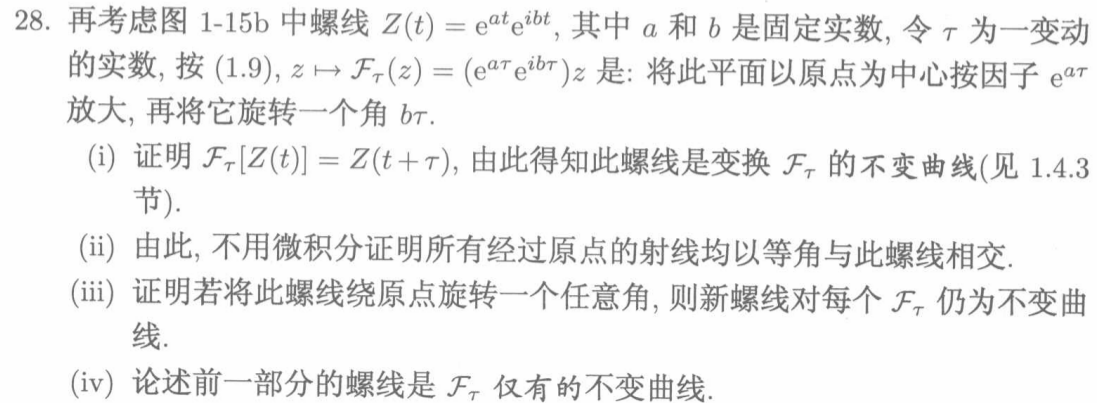
\includegraphics[width=1\textwidth]{/home/luqing/math/visual-complex-analysis/exercise1-5-28.png}
\begin{remark}
  值得指出的是,此处的翻译有问题,应该翻译成“将此平面旋转一个角$b\tau$,
  再以原点为中心按因子 $e^{a\tau}$ 放大”.
\end{remark}
\begin{proof}[\textbf{证明}]
(i)为了证明螺旋线是某个变换的不变曲线,只用证明螺旋线上的点经过该变换后
还在螺线上即可.我们考虑螺旋线的极坐标形式 $r=e^{(a/b)\theta}$,对于螺旋
线上的任意一点 $(e^{(a/b)\theta},\theta)$,将之逆时针旋转 $b\tau$ 后,变
成 $(e^{(a/b)\theta},\theta+b\tau)$.再以原点为中心按因子 $e^{a\tau}$放
大后,变成 $(e^{(a/b)\theta+a\tau},\theta+b\tau)$,易得该点仍然在螺线上.\\
接下来的全部省略.
\end{proof}
\end{document}








